\documentclass[10pt,twocolumn]{article}
\usepackage{fullpage}
\usepackage{times}
\usepackage{amsmath,proof,amsthm,amssymb,color}
%\usepackage{multicol}
\usepackage{float}
\usepackage{graphicx}
\floatstyle{boxed} 
\restylefloat{figure}
\usepackage{hyperref}
\usepackage{listings}
%\usepackage[all]{hypcap}


\title{virtexsquared: ARM-like System-on-Chip on an FPGA}

\author{Joshua Wise\\
\texttt{$<$jwise@andrew.cmu.edu$>$} \and
Josiah Boning\\
\texttt{$<$jboning@andrew.cmu.edu$>$} \and
Bradley Yoo\\
\texttt{$<$bjy@andrew.cmu.edu$>$}}


\begin{document}
\maketitle

\begin{abstract}

The authors provide an update as to the ongoing development of an ARM-like
System-on-Chip built on a Xilinx Virtex-5 FPGA.  A high-level overview of
the design is provided, as well as detailed examinations of various
submodules within the system.  The status of the project schedule is briefly
touched on.

\end{abstract}

\vspace{0.1in} % fff fu LaTeX

\section{Introduction}

In fulfillment of the 18-545 Advanced Digital Design Capstone, this group
is designing and implementing a peripheral layer for an ARM-like core. 
The system is built around two memory buses, and contains I/O cores to
interface with a smattering of peripherals, including:

\begin{itemize}
\item{DVI/VGA output from Chrontel CH7301C; video output will be cached in a
framebuffer in main memory.  Various acceleration primitives will be added
as needed for performance.}
\item{AC'97 audio with Analog AD1981B; audio buffering will be performed in
a simple main memory ring buffer.}
\item{PS/2 keyboard.}
\item{CompactFlash via the Xilinx SystemACE controller; software running on
the core will be capable of reading the filesystem on the CompactFlash
module.}
\item{DDR2 SODIMM; interface glue is provided using Xilinx's predesigned
Memory Interface Generator (MIG) IP.}
\end{itemize}

The system's functionality will be demonstrated using a small game. We
endeavor to produce a minimalistic clone of Dance Dance Revolution, with the
PS/2 keyboard used for input.  Assets will be taken from the open-source
game Stepmania.  The game will be loaded (and the core proven) using the
open-source bootloader U-Boot.  If time permits, Linux will be booted on the
core.

A side goal of this peripheral layer is to be reused in 18-447; the system
is designed to be simple to interface with from a core perspective, and
hence usable for students in an introductory computer architecture class. 
The core, in particular, has a moderate \textit{anti}-goal of high
performance; if there is time for high performance, it should be applied to
adding additional peripherals.

\section{Memory Architecture}

The system, as a whole, is partitioned into two major access paths -- the
FSAB (\textit{Fast System Access Bus}), and the SPAM Bus (\textit{Slow
Peripheral Access Memory} Bus).  These two buses were designed to meet
wildly differing goals; the FSAB is designed for high-bandwidth, cachable
transactions, whereas the SPAMBus is designed for configuration space
register (CSR) accesses.  Ideally, most of the system's traffic will occur
over the FSAB.

\begin{figure}
  \centering
    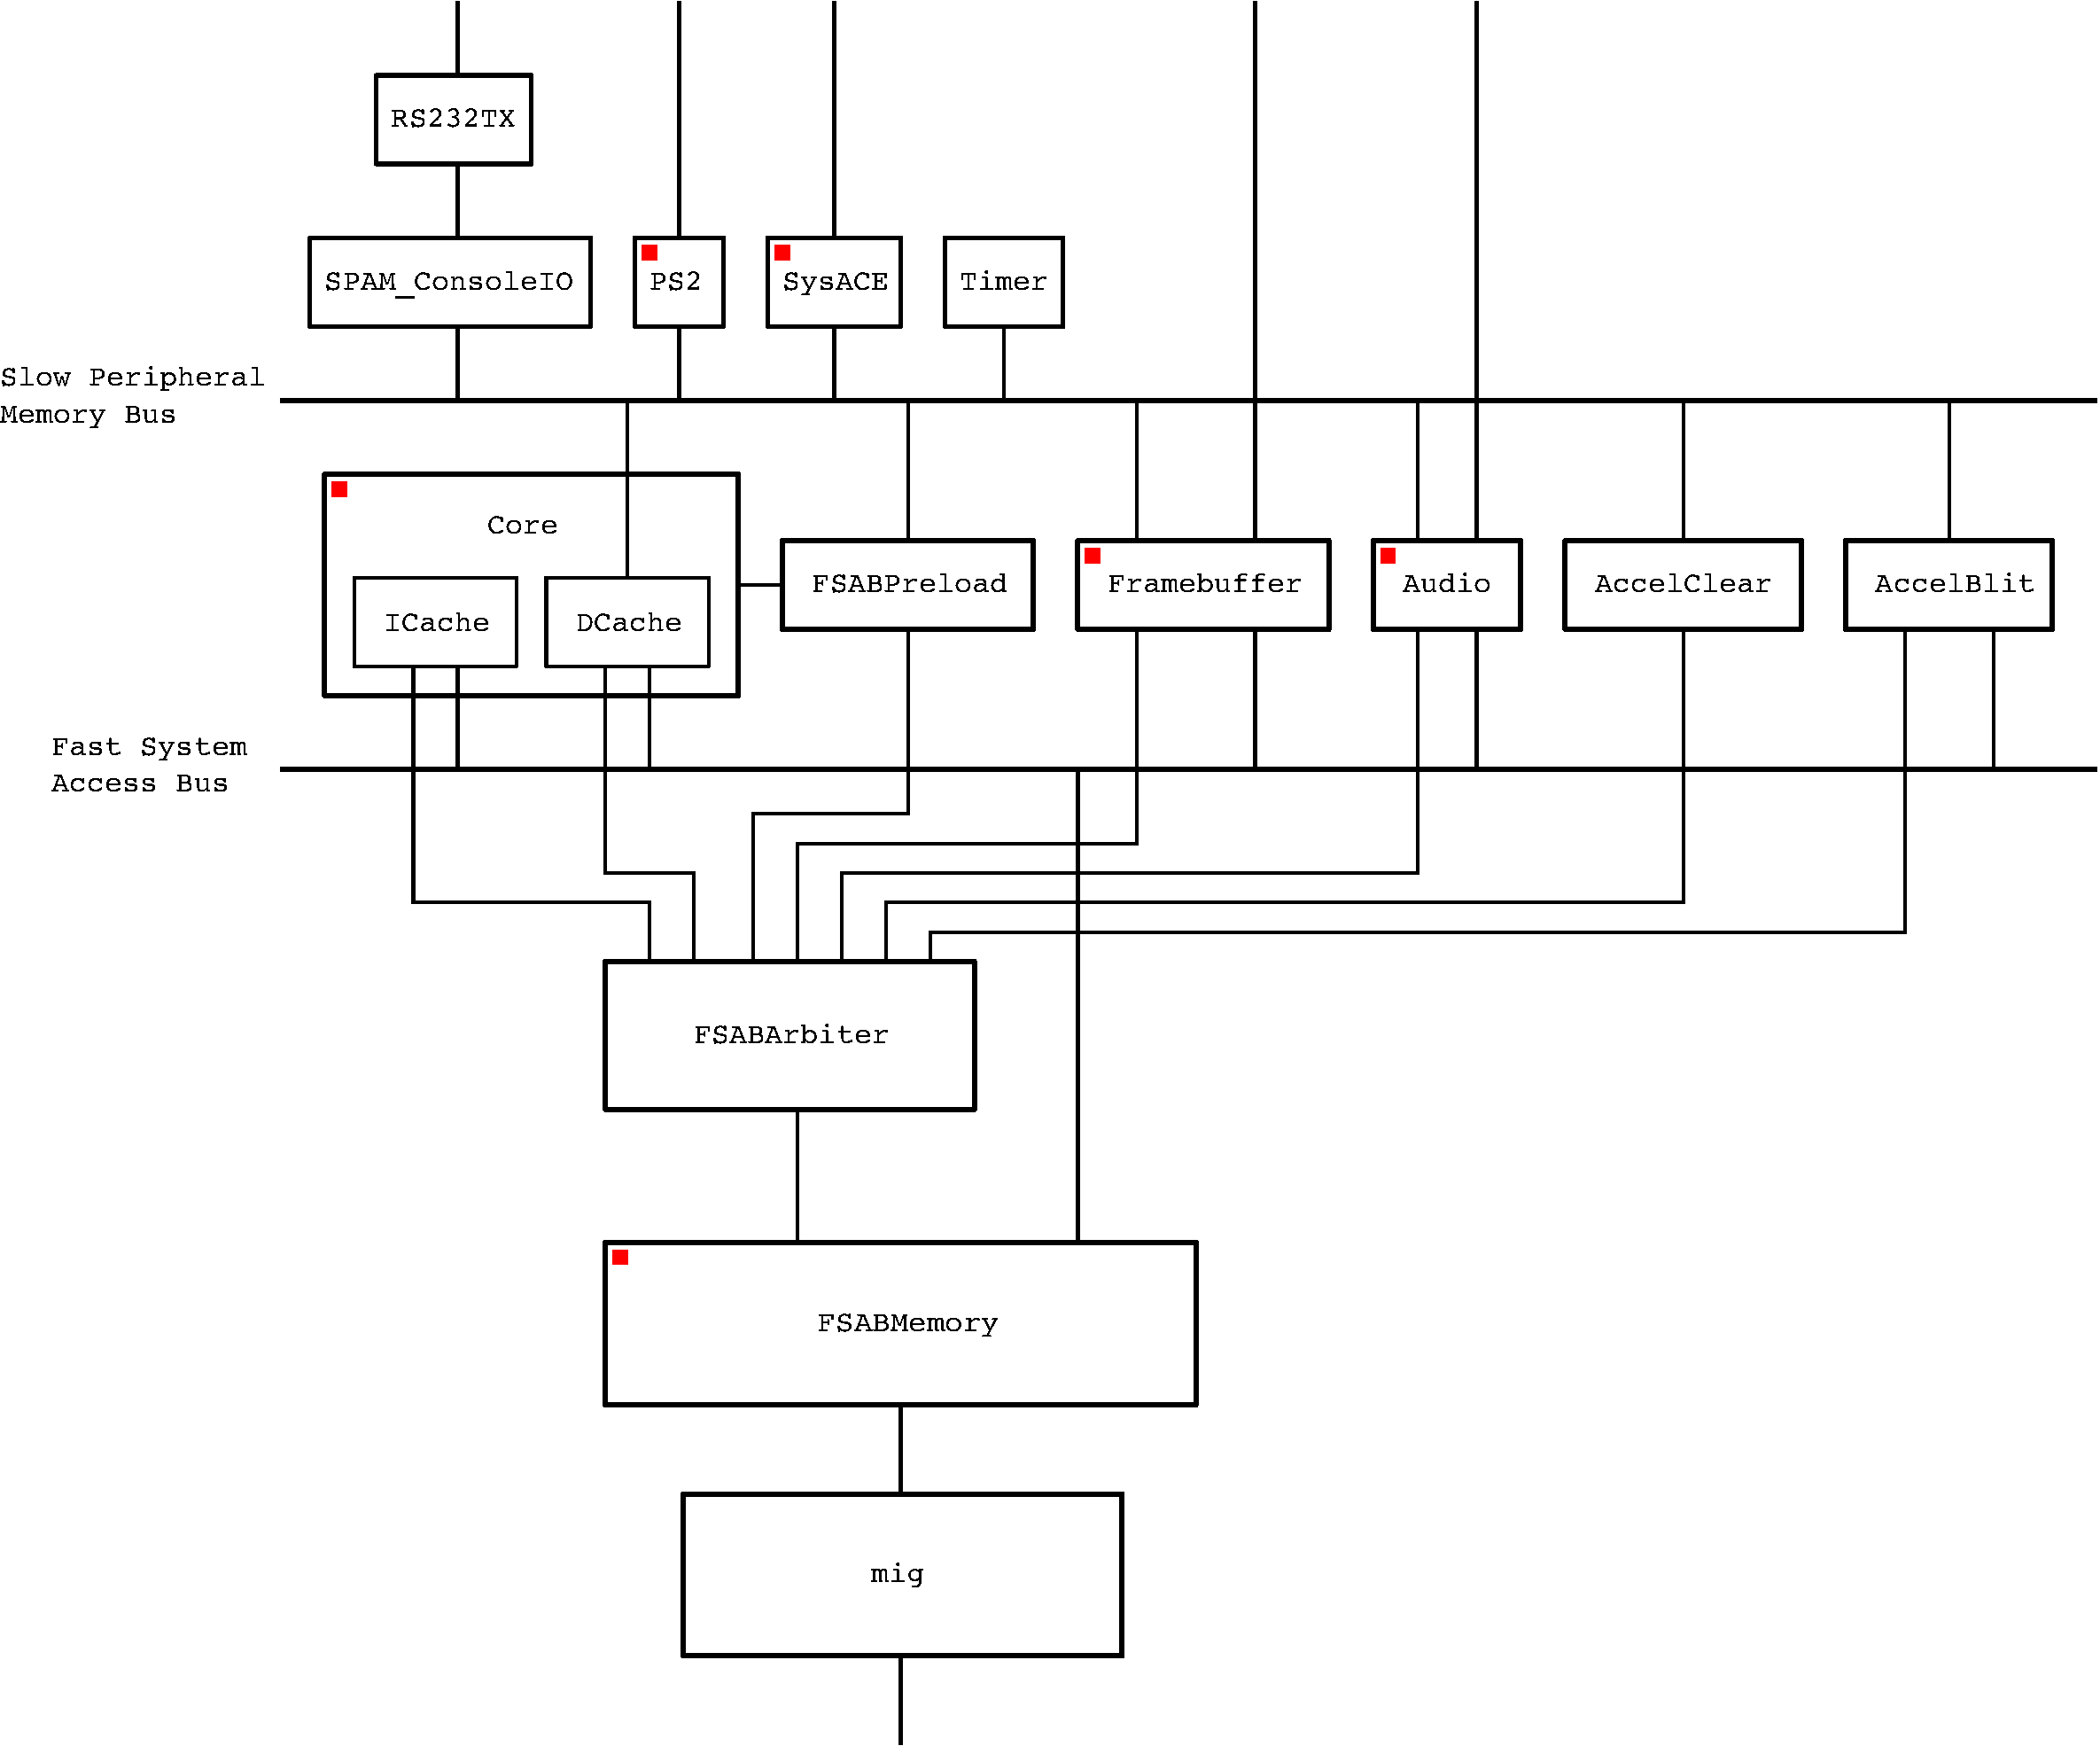
\includegraphics[width=0.49\textwidth]{block_diagram.pdf}
  \caption{High-level system diagram.} \label{system_diagram}
\end{figure}

\subsection{Fast System Access Bus}

The FSAB is a transaction-oriented bus designed primarily for accessing
high-latency memories such as DRAMs. The vast majority of the memory
accesses on the system during normal operation (i.e., not at
boot/configuration time) will happen via the FSAB.

\subsubsection{Terminology}

The FSAB works in terms of `transactions'. A read transaction shall consist
of the `read request', and `read data' phases. A write transaction shall
consist only of the `write data' phase.

Devices attached to the FSAB are classified as `masters' and `slaves'; a
device that initiates transactions (reads and writes to main memory) is a
master, and a device that completes transactions is a slave.

At times, it may be useful to discuss directions on the FSAB. For the
purposes of this discussion, data that is traveling from a master to a slave
is considered `outbound', and data that initiates at the slave and returns
to a master is considered `inbound'.

\subsubsection{Conceptual Overview}

virtexsquared, in its first incarnation, will only have a single memory
controller. For that reason, the FSAB will be defined to have only one slave
device - but since many peripherals may wish to do DMA access to or from
main memory, the FSAB will be defined to potentially have many masters. The
fact that only one slave device exists shall not be extensively exploited in
either the design or implementation of the FSAB, since at a later time, a
second memory controller may be interesting.

Since many memory controllers are capable of handling multiple pipelined
requests, the FSAB supports multiple transactions in flight at a time.  The
slave will arbitrate these requests with a debit-credit system.  Similarly,
contention between masters will be resolved with an arbiter module that also
performs queueing and debit-credit arbitration.  In this regard, the bus
arbiter should be ``invisible'' to a master; the debit-credit system should
be interface-identical as if the master were talking directly to the slave.

Most operations that peripherals on the FSAB will perform will be in similar
sizes.  For instance, the I\$ and D\$ will always read sizes of a single
cache line; the TLB will generally read page directory entries at a time;
and the framebuffer will generally load half a FIFO's worth or so at a time. 
The general case, anyway, will not be a read of a single word.  Similarly,
writes will often be localized to each other.  To facilitate this, each FSAB
transaction will have a count of words up to some defined maximum along with
the command and address.  The address shall autoincrement with each datum
sent.  Since not every datum may be interesting for a write, a "write mask"
should also be sent with every word written.

Since masters are isolated from each other by one or more arbiters, it is
generally not possible for one master to know what another master is doing. 
\footnote{This combined with the fact that writes happen on a delay -- that
is, when the memory controller gets around to it -- may pose a problem. 
Specifically, a program that writes to memory and then causes the cache line
to be read in again (or that kicks off a read on another device using the
SPAM) should be careful to verify that the write completes before the read
completes.  Depending on the specifics of the design and the ordering, this
may or may not be a problem, but it should be carefully considered.} Lacking
any other form of cache coherency protocols (such as MOESI), a system based
around the FSAB is not cache-coherent!  This means that the applications
programmer must take extra care to make sure that all data is synchronized
to main memory before allowing another peripheral to access said data.  (For
instance, if the programmer wishes to write new data to the frame buffer
before flipping pages, he must cause the CPU to clean that cache line by
some mechanism first.)

\subsubsection{Design Overview: Portlist}

A FSAB master has the following ports outbound:

\begin{lstlisting}[basicstyle=\footnotesize,language=Verilog]
output                  fsabo_valid;
output [FSAB_REQ_HI:0]  fsabo_mode;
output [FSAB_DID_HI:0]  fsabo_did;
output [FSAB_DID_HI:0]  fsabo_subdid;
output [FSAB_ADDR_HI:0] fsabo_addr;
output [FSAB_LEN_HI:0]  fsabo_len;
output [FSAB_DATA_HI:0] fsabo_data;
output [FSAB_MASK_HI:0] fsabo_mask;
input                   fsabo_credit;
\end{lstlisting}

A FSAB master has the following ports inbound:

\begin{lstlisting}[basicstyle=\footnotesize,language=Verilog]
input                   fsabi_valid;
input  [FSAB_DID_HI:0]  fsabi_did;
input  [FSAB_DID_HI:0]  fsabi_subdid;
input  [FSAB_DATA_HI:0] fsabi_data;
\end{lstlisting}

No debit output (or input) is needed; a debit occurs implicitly when a new
FSAB transaction is begun. The credit input is always considered valid, even
if the inbound valid flag is not set.

\subsubsection{Design Overview: Transaction Specifics}

Transactions are defined by a start packet (and potentially additional data
packets) being sent to a slave, and the slave responding with any necessary
data packets. The slave may pipeline transactions as much as it is able
(credits can be returned before the slave has responded), but the slave
shall never reorder transactions. (Doing so would result in indeterminate
behavior with reads after writes, among other things.)

A start packet shall consist of the valid bit being set, the mode flag being
set to either FSAB\_READ or FSAB\_WRITE, the did/subdid set to the appropriate
values, an address, a length, and the first word of data and mask, should
they be valid for the current operation. Once a transaction is being sent
outbound, it shall not be interrupted by another transaction; the next data
packets are always part of this transaction. (For this reason, a master
should attempt to send packets as quickly as possible; excessive delay
between subsequent assertion of the valid flag may result in poor bus
performance.) In subsequent data packets, all control flags (i.e., all but
valid, data, and mask) are ignored.

The debit/credit system shall count each transaction as a debit, not each
word. Another transaction may be sent immediately after the credit flag is
asserted (or the credit may be queued).

The did field of each transaction shall be set as per each master's DID
assignment. The subdid may be set according to any internal state that the
master needs to track.


\subsubsection{Known implementations}

The following are known implementations of the FSAB specification:

\begin{figure}
  \centering
    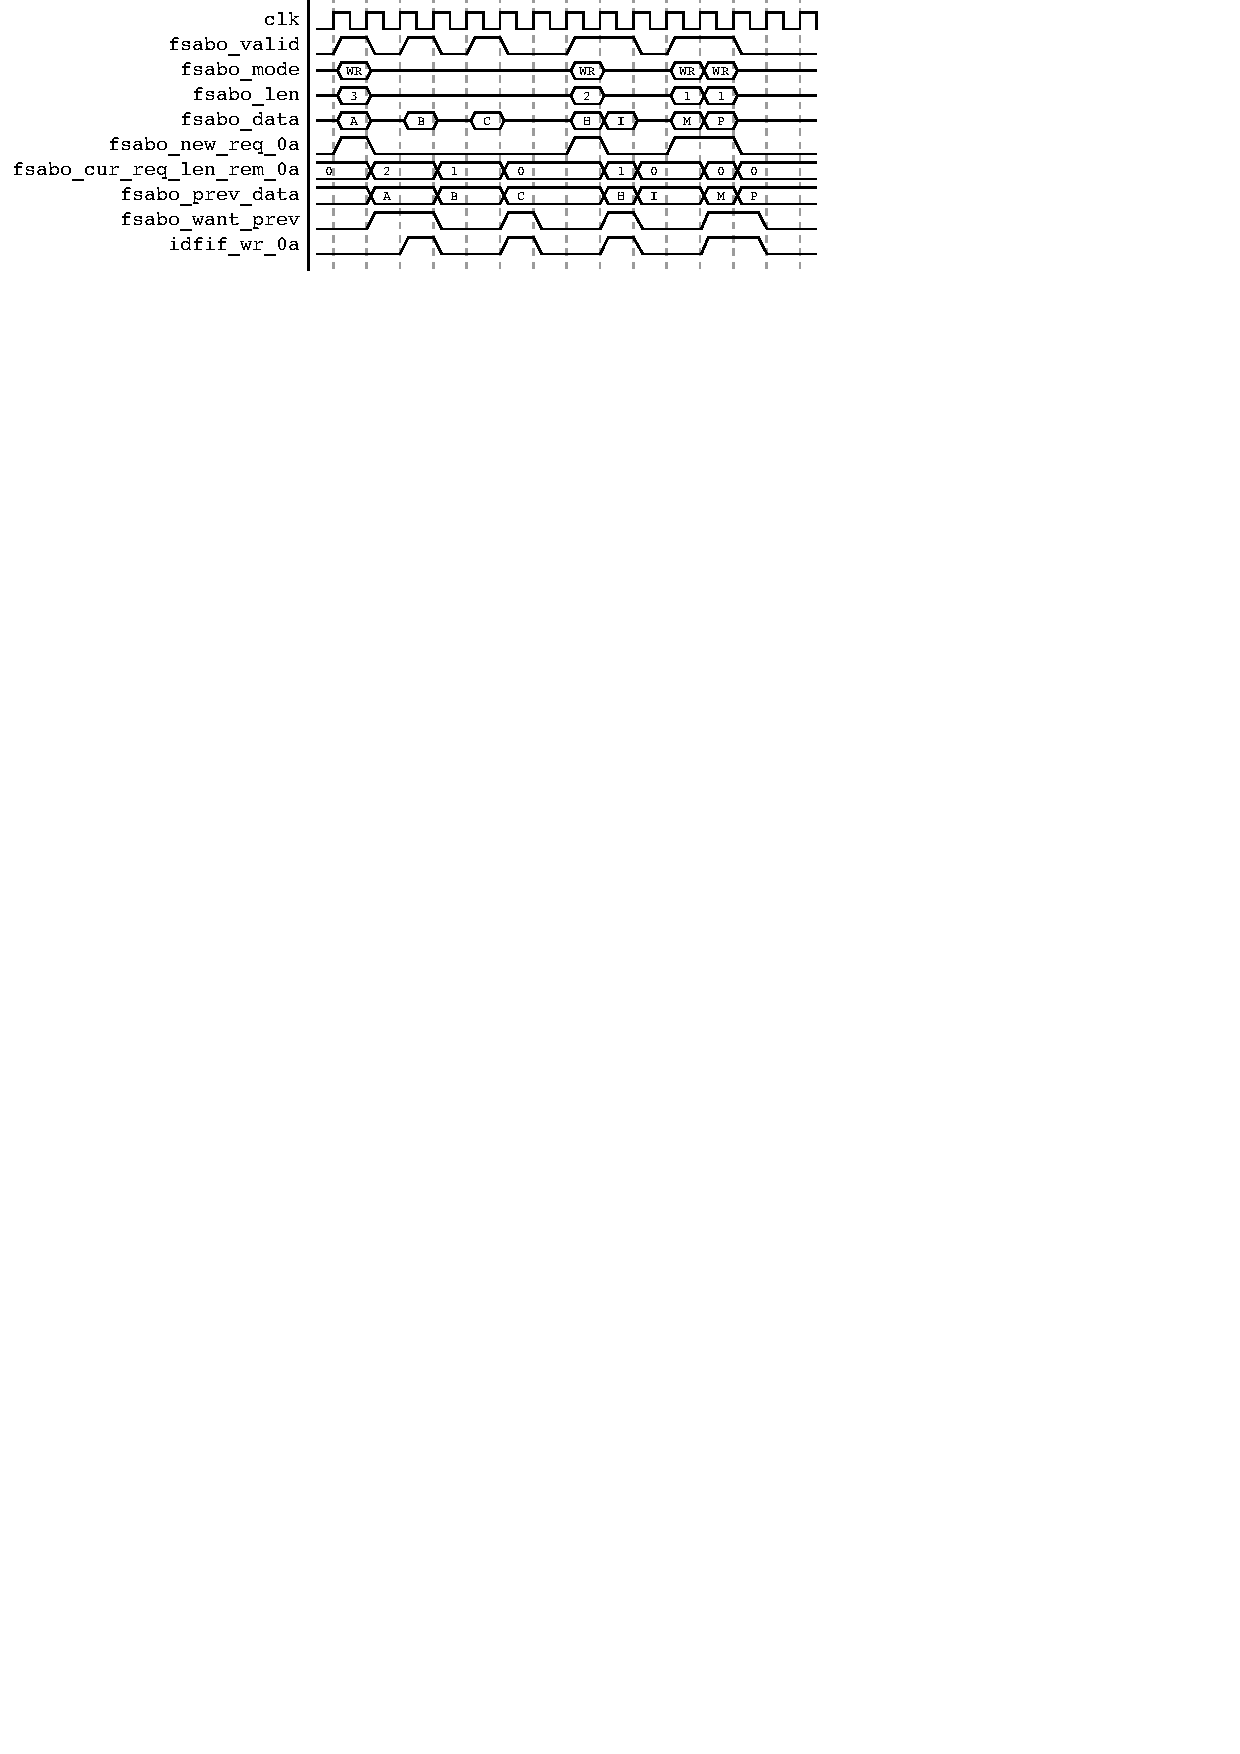
\includegraphics[width=0.49\textwidth]{FSAB-IxFIF.pdf}
  \caption{Clocking for memory controller.} \label{mshim_clock}
\end{figure}


\begin{itemize}
\item{Caches}
\item{Memory Controller}
\item{Arbiter}
\item{DMA Controller}
\end{itemize}

\subsection{Slow Peripheral Access Memory}

The SPAM bus is a word-oriented one-access-at-a-time bus designed primarily
for accessing configuration space registers (CSRs) on peripherals.

\subsubsection{Conceptual Overview}

In theory, all peripherals on the system will be matching and decoding on
the SPAM bus; when the processor does a SPAM-bus access, it is almost
certainly the case that a device will respond.  So, the bus should be
optimized for the common case in which a device responds shortly after a
request is sent.  Similarly, it should be the case that only one device ever
matches, so the bus need not be arbitrated between them; a simple OR'ing of
responses should work.

No peripheral should need to access any other peripheral's CSRs; any such
accesses from a debug interface should be multiplexed in between the CPU and
the SPAM-bus.  As such, the master-slave relationship in the SPAM-bus is
exactly the opposite of what it is on the FSAB; there is only one SPAM-bus
master, and there can be many SPAM-bus slaves.  Again, this property should
not be extensively exploited, but it is the case in the current
implementation.

Requests on the SPAM-bus should ordinarily be low latency, but there may be
need for wait states for various reasons.  For instance, if the other
peripheral is far away on the die, it may take an extra clock to compute the
appropriate response for a read.  A write, perhaps, may block until some
(short) action is complete.  There may also be a need to block because the
target peripheral is in a different clock domain, and a synchronizer needs
to shift the data over.

If no peripheral answers by deasserting busy\_b within a reasonable number
of cycles (usually 256), the request is deemed to have timed out, and a read
should return a value indicating that (usually something along the lines of
0xDEADDEAD).

\subsubsection{Design Overview: Portlist}

The processor has the following ports outbound:

\begin{lstlisting}[basicstyle=\footnotesize,language=Verilog]
output                  spamo_valid;
output                  spamo_r_nw;
output [SPAM_DID_HI:0]  spamo_did;
output [SPAM_ADDR_HI:0] spamo_addr;
output [SPAM_DATA_HI:0] spamo_data;
\end{lstlisting}

The processor has the following ports inbound:

\begin{lstlisting}[basicstyle=\footnotesize,language=Verilog]
input                   cio__spami_busy_b;
input  [SPAM_DATA_HI:0] cio__spami_data;
\end{lstlisting}

\subsubsection{Design Overview: Lifecycle of a request}

A request begins by the processor asserting the valid flag and specifying
the rest of the fields. This happens for exactly one cycle. Some time later
(potentially even on the same cycle), a device may assert the busy\_b flag
for one cycle to indicate that the request has been filled. Inbound data
shall be valid on the same cycle.

No new request shall be specified until either a previous request has
returned, or a previous request has timed out. A request shall time out
after no fewer than 128 cycles.

When a device is not specifying data inbound, it shall drive its output port
to zero, so that all data ports can be safely OR'ed together.

\section{Core Microarchitecture}

is a hilariously bad disaster.  Let us never speak of it again.

\section{Peripheral Architecture}

is another section to be filled in.

\section{Tools}

virtexsquared is developed using some standard tools, and some custom tools. 
The parts of the virtexsquared development system that appared to be of
particular use are elucidated below.

\subsection{Xilinx XST}

\subsection{verilog-mode}

\subsection{GNU make}

\subsection{makecdc for ChipScope}

\subsection{git}

\section{Schedule}

Gantt chart is figure 3.  We are behind it.  I ran out of time to write
this because I spent all night debugging.

\begin{figure*}
  \centering
    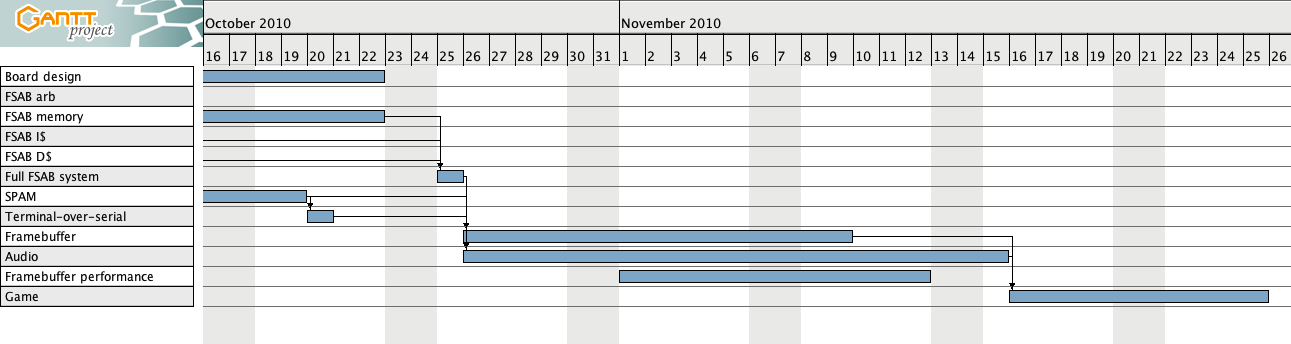
\includegraphics[width=\textwidth]{gantt-chart.png}
  \caption{I hate Xilinx.} \label{mshim_clock}
\end{figure*}


\end{document}
